%stap

\documentclass[../../main/main.tex]{subfiles}


\begin{document}
\title{Systems-theoretic Process Analysis}


\chapter{Systems-theoretic Process Analysis}
\section{Systems Engineering}
\section{Systems Security Engineering}
\section{Systems-theoretic Process Analysis}
\section{STPA Overview: Four Steps}
\section{STPA on Patrol Base Operations}
\subsection{Define The Purpose of The Analysis}
\subsection{Model The Control Structure}
Defining the system boundaries: (reference Ranger Handbook)
One of the challenges in modeling the patrol base operations is generality.  Patrol base operations may consist of a fire team comprised of ? soldiers, a platoon comprised of ? soldiers, or something in-between.  The mission may be to engage with the enemy, to acquire intelligence for the main body, or some else.

\footnote{Note that the Ranger Handbook specifically states that "because a patrol is an organization, not a mission, it is not correct to speak of giving a unit a mission to "patrol.""  The term "mission" used in this master thesis refers generally to the mission (or objectives) of the patrol base operations, and does not refer to the patrol as being a mission.}

Figure \ref{system} shows a diagram relating a system to its boundaries, subsystems, and inputs and outputs.  These each described below.

\begin{figure}[h]
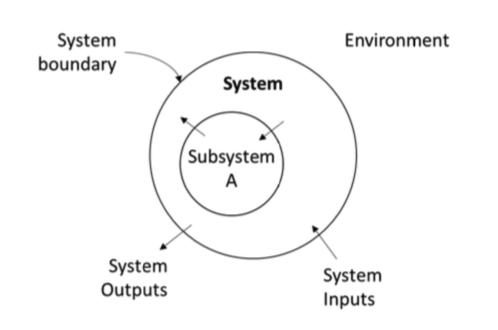
\includegraphics[width=\linewidth]{../figures/system}
\caption{\label{system}Relationship of system to system boundaries, subsystems, inputs, and outputs. (Image from \glsentryshort{nist} Special Publication 800-160: Systems Security Engineering Considerations for a Multidisciplinary Approach in the Engineering of Trustworthy Secure Systems.)}
\end{figure}
\paragraph*{System}
In this master thesis, the "system" refers to a platoon-sized patrol base operation.  This is the best choice because a platoon-sized operation may be scaled-down to accommodate a squad-sized or fire team-sized detachment, but not the other way around. 

The mission details are intentionally kept vague to accommodate as many types of missions as possible.  The system boundaries for the model are the start and end of the mission. In this master thesis, the patrol base operations begin in the planning phase when the patrol leader receives the mission.  The patrol base operations end after the patrol withdraws from the operations and returns to the main body\footnote{Completion should include reporting to the commander.  However, for the purposes of this master thesis, it was sufficient to conclude a withdraw.  Nevertheless, with our model of the patrol base operations, it is easy to add a phase for reporting to the commander.}

\paragraph*{Subsystem}
A subsystem in the patrol base operations is any smaller group of soldier assigned to a specific task such as security or reconnaissance.  This may include a squad or fire team.  

\paragraph*{Environment}
The mission is determined by the greater-wisdom of the U.S. Army leadership at the time of need.  This means that environmental boundaries, mission boundaries, and other system requirements must be determined by the patrol leader  (referred to as the platoon leader in other chapters) after the mission is received and during the planning phase.  For this reason, STPA analysis should be performed on a mission before it is referred to the patrol.  But also, patrol leaders should be trained in STPA to make a quick and accurate analysis of mission-specific system boundaries.  


\paragraph*{System Inputs and Outputs}
The system input is the mission handed down by the U.S. Army leadership.  Additional inputs such as equipment, weapons, and additional personnel are determined when the mission is received. 

System outputs are mission dependent.  They may be successful engagement with the enemy, the capture of an enemy combatant, acquisition of specific intelligence, or anything else defined by the mission objectives.




\subsection{Identify Unsafe Control Actions}
\subsection{Identify Loss Scenarios}
\end{document}